\documentclass[12pt,a4paper]{article}
\usepackage[utf8]{inputenc}

\title{Mémoire Master 2 MIAGE}
\author{HAJ ISMAIL Mohamed}
\date{May 2017}
\usepackage{pifont}
\usepackage{fancyhdr}
\pagestyle{fancy}
\fancyhf{}
\fancyhead[L]{\rightmark}
\fancyhead[R]{\thepage}

\setlength{\headsep}{0.6in}

\usepackage{engrec}

\usepackage[utf8]{inputenc}
\usepackage[toc,page]{appendix} 
\usepackage{color}
\usepackage[usenames,dvipsnames]{xcolor}
\usepackage{euscript}
\usepackage{amsmath}
\usepackage{amssymb}
\usepackage{amsfonts}
\usepackage{dsfont}
\usepackage{graphicx}
\usepackage{verbatim}
\usepackage[francais]{babel}
\AddThinSpaceBeforeFootnotes % à insérer si on utilise \usepackage[french]{babel}
\FrenchFootnotes 
\usepackage{epsfig}
\usepackage{thmbox}
\usepackage{graphicx}

\usepackage{amssymb}
\usepackage{caption}

\usepackage[final]{pdfpages}
\usepackage[export]{adjustbox}
\usepackage{afterpage}
\usepackage{emptypage}
%\usepackage{moreverb}
\usepackage[toc,page]{appendix} 
\usepackage{a4wide}
\usepackage{csvsimple}
\newcommand{\R}{\mathbb{R}}
\newcommand{\Q}{\bf{Q}}
\usepackage{float,lscape}
\usepackage[nottoc]{tocbibind}

\usepackage[francais]{babel}
\usepackage[T1]{fontenc}
\usepackage{listings}
\usepackage{caption}
\usepackage{subcaption}

% Length to control the \fancyheadoffset and the calculation of \headline
% simultaneously

%\renewcommand{\headrulewidth}{0pt}


\usepackage[letterpaper, margin=1.5in]{geometry}



\newcommand{\espace}{\vspace{0.3 cm}}


\begin{document}
\begin{titlepage}
\begin{figure}[h]
    \begin{minipage}[c]{.16\linewidth}
        \centering
        
\includegraphics{logouniv}
    \end{minipage}
    \hfill%
    \begin{minipage}[c]{.16\linewidth}
        \centering
        
\includegraphics{segmi}
    \end{minipage}
\end{figure}
\begin{center}
\textsc{\Large $2^{\grave{e}me}$ années de Master Méthodes Informatiques Appliquées à la Gestion des Entreprises \textbf{MIAGE} }\\[0.5cm]
% Title

{ \huge \bfseries Mémoire de fin d'étude \\ 2016-2017   \\[0.4cm] }

\noindent\rule{12cm}{0.4pt}

\vspace{0.5cm}

\Large {La réorganisation de l'entreprise peut-elle remettre en cause l'agilité d'un service?} 

\vspace{0.3cm}

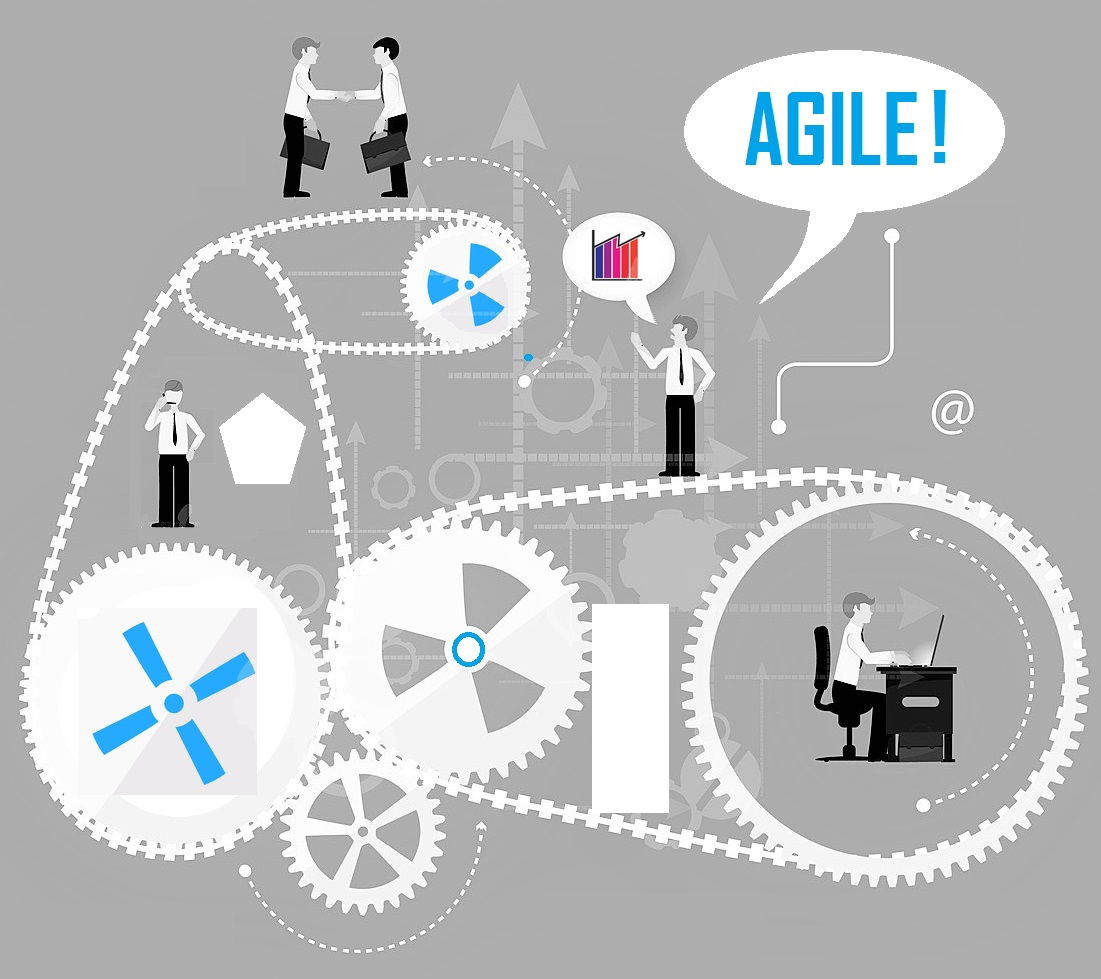
\includegraphics[width=0.5\textwidth]{agile.jpg}~\\[1cm]

\end{center}

\begin{flushleft}
 \Large \textbf{Auteur :} 
\textsc{HAJ ISMAIL} Mohamed \\


\definecolor{segmicolor}{RGB}{119,189,238}
\emph \large \textbf{\color{segmicolor}Tuteur\,:} 
 \textsc{PRADAT-PEYRE} Jean-François
 
\end{flushleft}

\end{titlepage}
 
\newpage
\thispagestyle{empty}
\strut 

\newpage
\setcounter{page}{3}
\textbf{\huge Remerciements}



\vspace{1.5cm}

\hspace{0.5cm} 

Je tiens à remercier l’ensemble de l’équipe du data management commercial de Philips pour avoir, contribué, par tous les moyens possibles, au bon déroulement de mon projet. De plus, je les remercie pour leur chaleureux accueil, leur bonne humeur ainsi que pour tous les conseils qu’ils m’ont fournis.

Pour l’expérience enrichissante et pleine d’intérêt que j’ai pu vivre durant ces cinq mois dans le service de Data Management de Philips Lighting, je tiens à remercier tout particulièrement et à témoigner toute ma reconnaissance aux personnes suivantes :\\

Merci tout particulièrement à Monsieur \textbf{Philippe DEMANGE}, responsable de l’équipe de Data Management EMEA, de m’avoir donné l’occasion d’effectuer mon stage au sein de la société Philips, pour son accueil et la confiance qu’il m’a accordé dès mon arrivé dans l’entreprise.\\

Merci également à Madame \textbf{Sylvie Moumen}, Monsieur \textbf{Christophe FLORISSONE} ainsi qu'aux différents membres du Data Management rencontrés pour leur disponibilité et leur cordialité. \\

Merci aussi à \textbf{Jean-François PRADAT-PEYRE} pour son aide dans la rédaction de ce mémoire ainsi que pour les cours dispensés ces dernières années dans le cadre de la formation MIAGE.\\

De plus, je remercie le corps enseignant de la MIAGE de Nanterre pour les enseignements qui m'ont été dispensés ces trois dernières années. Ainsi qu'à l'équipe \textbf{ReviZ Team} composée de \textbf{Bruno VERALDI}, \textbf{Leyla ELATTAR} ainsi que d' \textbf{AMEL BRAHIMI} pour leurs soutiens tout au long de l'année. Ils ont été d'une grande aide lors des révisions de même pour la rédaction du mémoire.\\

Enfin, je remercie tous mes proches pour leur patience et leur soutien inconditionnel.


\newpage
\thispagestyle{empty}
\strut

\newpage
\tableofcontents

\newpage
\part{Introduction}

Sous l'effet d'une évolution constante de l'environnement économique, les entreprises sont soumises à de multiple processus de réorganisation. Ces faits observés sont des processus qui ont pour but de trouver de la flexibilité ainsi que des avantages compétitifs, tel que les réorganisations interne, les réductions du personnel, ou encore les modifications de processus. Dans un contexte où certains événements se produits tel que le PSE \footnote{"Plan de Sauvegarde de l’Emploi"}, fusion, changement organisationnel important, une nouvelle direction ou tout simplement suite à une crise, ceci va prendre une dimension particulière à cause de leur ampleur. Dans de multiple cas, elles résultent de décisions stratégiques et de choix de gestion.\\

Les journalistes évoquent beaucoup l'actualité des réorganisations de plusieurs secteur économique. Pour le journal 20 minute, « Le groupe ENGIE vivant un vaste plan de transformation. Il présentera cette restructuration aux instances locales. Interrogé par l’AFP, le géant français de l’énergie a simplement confirmé qu’un « projet de nouvelle organisation du siège est présenté aux instances représentatives du personnel du groupe ».
« Cette évolution reposera sur le seul principe du volontariat et ne conduira à aucun licenciement », a précisé ENGIE. Des négociations sont déjà en cours sur les mesures d’accompagnement, ont précisé les sources syndicales. Le fournisseur français d’électricité et de gaz travaillait depuis cet automne sur la restructuration des services RH, juridique, marketing ou encore finances. Les suppressions de postes annoncées représentent 30 \% de l’effectif dédié en France, 50 \% en Belgique et 100 \% au Royaume-Uni. »\\

Pour le dirigeant d’entreprise, l'un des enjeux majeurs est de clarifier sa vision à moyen et long terme, de définir les investissements les plus pertinents, afin d’améliorer les performances métier, de pouvoir saisir toutes les opportunités et d’atteindre ses objectifs stratégiques. Comme l'a évoqué le 20 minutes concernant la société AirBus : « Le plan de restructuration baptisé « Gémini » prévoit la fusion de la branche aviation commerciale (Airbus SAS) et du reste du groupe (Airbus Group). Elle doit être effective à l’été 2017 et doit permettre selon la direction d’éviter les « duplications » de postes et de gagner en « agilité ». » Mais bien que le dirigeant définisse une stratégie, il aura du mal à la faire appliquer sans un management actif à tous les niveaux.\\

Les entreprises gagne de plus en plus en agilité. Dans une économie mondialisée de plus en plus concurrentielle, les sociétés se doivent d'être agiles, pour pouvoir aborder comme il se doit le changement. Comme l'énonce le 20Minutes pour le groupe PSA : « L'entreprise «doit se protéger et assurer sa pérennité, et celle de l'emploi de ses salariés, en s'appuyant sur l'excellence opérationnelle, la performance et l'agilité». ».\\


Mais, l'agilité ne revendique pas être une solution suprême et prêt à l'emploi pour tous les problèmes liés à la transformation. Il est plutôt un ensemble de principes et de techniques qui va permettre à chacun de manipuler avec plus de flexibilité et de plaisir.\\


Un questionnement est donc naît de cette introduction ainsi qu'à la suite des deux précédents stages effectué dans des entreprises subissant une réorganisation. La problématique est à savoir si :\\
\begin{center}
« \textbf{La transformation d'une entreprise peut elle remettre en cause l'agilité d'un service?} »\\
\end{center}



Afin d’essayer de répondre à cette question, nous verrons tout d’abord les raisons qui poussent les entreprises à vouloir faire une transformation de leur entreprise, ensuite nous étudieront le besoin d’agilité des entreprises, puis nous ferons le point sur les interactions entre la réorganisation et l’agilité avec des exemples de projets et conclure sur la façon d’allier la restructuration et l'agilité.

\newpage
\thispagestyle{empty}

\part{Etat de l'art}

\section{La Transformation}

La transformation d'une entreprise se fait de façon structuré et sans précipitation. Pour beaucoup de chercheur la transformation est synonyme de « changement », « débureaucratiser », ou même « modification significative » . Ce qu'il faut savoir c'est que la réorganisation fait partie de la transformation. Si l'entreprise est agile cela rendra la transformation de la compagnie plus aisée.

Dans cette partie, nous verrons ce qu'est une transformation ensuite nous aborderons la chronologie historique de la transformation. Enfin nous verrons le lien entre la transformation et l'agilité.


\subsection{Qu'est ce que la transformation}


La transformation dans le milieu de l'entreprise peut être considéré comme une restructuration, à commencer le Larousse qui précise que la transformation est un changement de façon radical d’un état à un autre. Tout comme la métamorphose de la chenille en papillon en passant par la chrysalide, qui sera traité un peu plus tard. Quant à la restructuration c'est une action de réorganiser, selon de nouveaux principes, un ensemble que l'on juge inadapté. Au delà d'une identification par défaut, de multitude explication et principe permettent de comprendre ces cas de figures, d'en juger l'évolution dans le temps et son envergure, et finalement d'en exposer la dimension devenue universelle, permanente, et protéiforme.\\

%Pour réaliser ses ambitions et atteindre ses objectifs, l’organisation agile implique de replacer l’Humain au centre de l’organisation. Pour que chacun donne le meilleur de lui-même.

Diffuses, permanentes, protéiformes, omniprésentes… tels sont les principaux qualificatifs attribués par les chercheurs aux restructurations. Ces qualificatifs peuvent changer lorsque s’expriment des représentants de directions qui, par exemple, les jugent inévitables, incontournables ou encore naturelles car « faisant partie de la vie des entreprises ». \footnote{(Rachel Beaujolin-Bellet,  Géraldine Schmidt, Introduction, La Découverte « Les restructurations d’entreprises », 2012, p. 3)}\\

Toutefois, la restructuration ne veut pas toujours dire la réduction du périmètre de la firme. Ici, la définition proposée par E. Bowman et H. Singh (1993), présente la restructuration comme « l'ensemble des transactions conduisant à vendre ou à acquérir des actifs, à modifier la structure du capital et à transformer l'organisation interne de la firme »\footnote{Can encompass a broad range of transactions, such as selling business lines, making significant acquisitions, changing the capital structure through an infusion of debts, or altering the internal organisation of the firm}. D'après Beaujolin-Bellet,  Géraldine Schmidt, la « restructuration », très imparfaitement appréhendée en termes statistiques, proche de bien d’autres notions, souvent simplement assimilée à une opération de suppressions d’emplois ou à un plan social, mais renvoyant plus largement à des transformations internes et externes de la structure organisationnelle, à des modifications significatives de l’organisation du travail et/ou à un changement de la relation d’emploi et des modalités de gestion de cet emploi. Cet effort de précision et de cadrage conduit alors à décrire la multiplicité des manifestations ou des formes de restructurations, et à distinguer plusieurs registres ou logiques de décisions possibles. Restructurer une organisation relève d’une décision »\\
 
D’autres termes sont souvent identifiés à celui de la restructuration, et il convient d’en clarifier les définitions. Selon un rapport du Bureau International du Travail [Rogovski et al, 2005], le mot restructuring est l'un des termes le plus couramment utilisés dans le monde anglo-saxon. Olivier Furrer, le 13 avril 2016, pour organiser le large éventail des activités de restructuration existantes, on peut distinguer trois types principaux : une restructuration du portefeuille d’activités, une restructuration financière, ou une restructuration organisationnelle. \\
\newpage
\begin{figure}[h!]
\centering
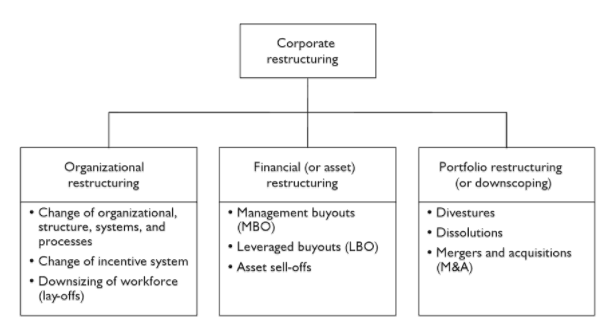
\includegraphics[scale=1]{restructuration}
\caption{Structure et éléments de restructuration d'entreprise par Bowman et Singh, 1993}
\label{fig:graph}
\end{figure}
 
La restructuration du portefeuille « Portfolio restructuring » implique une suite d'acquisitions et de désinvestissements qui modifiera la configuration des activités de l'entreprise.

%Portfolio restructuring also involves a sequence of acquisitions and divestitures that will change the configuration of the firm's businesses
 
Alors que la restructuration financière « Financial restructuring » consiste plutôt à modifier la structure financière de l'entreprise et implique généralement l'apport de dettes en grandes quantité, que ce soit pour financer le rachat à effet de levier \footnote{C'est une technique financière d'achat d'entreprise.} (LBO), ou racheter des stocks d'investisseurs en actions ou payer de gros dividendes ponctuels.
 
%financial restructuring instead consists of change to the financial structure of the firm and usually involves the infusion of large amounts of debt, whether to finance leveraged buyout (LBOs), or buy back stock from equity investors, or pay large one-time dividends

Enfin, la restructuration organisationnelle « Organizational restructuring » tente d'accroître l'efficience et l'efficacité de l'entreprise grâce à des changements importants dans sa structure organisationnelle. Il est souvent accompagné de réductions de personnel et de licenciement de nombreux employés.\\

%Finally, organizational restructuring attempts to increase the efficiency and effectiveness of the firm through significant changes in its organization structure. it often is accompanied by downsizing and layoffs of many employees.
 
 
Tandis qu'en France, nous avons une multitude de vocabulaire lié à la transformation, et cela nous montre bien les différentes situation que nous pouvons avoir : réorganisation, refonte des process, délocalisation, fermeture de site, fusion, scission, cession...\\
 
Cette pluralité d'expressions énoncés, nous montre de la difficulté, relevé par Severin \footnote{Restructuration de l'entreprise - Théorie et Pratique (Broché)
Eric Séverin}, à s'associer sur une théorie de la restructuration.\\

Par conséquent, la transformation entraîne ainsi un changement organisationnel bien plus important que des changements courants. Elle touche au minimum toute une partie de l’organisation ou au plus l'ensemble de la société, et ne s'arrête pas à des changements secondaires de l’activité. Les modifications effectués peuvent s'expliquer par une fermeture, une réduction d’effectifs, l’externalisation, la sous-traitance, la fusion, la délocalisation de la production, la scission ce que subit actuellement la société Philips Lighting  ou toute autre réorganisation interne complexe.

%La réorganisation est une partie de la transformation. Si une entreprise fait juste une réorganisation cela veut dire que c'est une transformation incomplète ou alors cela ne l'est pas. Il y a eu un moment ou le service a un peu trop grandis, beaucoups de gens se reporte a un manager ce qui amenera a creer deux équipes ou le fusionner avec un autre. par exemple lorque Royal Philips et philips lighting dans la meme entité philips. EIM etait commun aux deux et lorsque philips lighting s'est séparé du groupe philips l'équipe EIM a été par la meme occasion séparée. les équipe étaient plus ou moins séparé mais il y a eu quelques personnes qui sont passées d'une équipe à une autre mais ce n'est pas une transformation car il n'y avait pas de rupture d'un etat à un autre.

\subsection{L'évolution historique}

La restructuration ne date pas d'hier, d'après Bernard Gazier « elle est aussi vieille que le capitalisme ». Les restructurations d’entreprises se sont multipliées depuis quatre décennies.\\ 

On peut constater qu'il y a deux types de mouvement restructuration:\\

La première serait une restructuration de crise dans les années 70-80 elles sont liées à une volonté de sauvegarder la société. Comme l'évoque Aggeri et Pallez (2005) considèrent que « jusqu’aux années 1970, les restructurations industrielles désignaient des phénomènes bien identifiés : elles concernaient un petit nombre de secteurs industriels dont l’adaptation paraissait douloureuse, mais inéluctable (textile, chantiers navals, sidérurgie…) ».\\

La seconde serait une restructuration de compétitivité qui aurait débuté dans les années 1990-2000. Cela concernent des compagnies qui ont une bonne situation économique, n'ayant pas de gros choc sur leurs marchés, mais inscrites dans une course à la performance, y compris financière, les amenant à restructurer par anticipation. D'après Marie Raveyre (2005) pour qui « désormais l’économie et les entreprises tendent à entrer dans un état durable d’instabilité : la recherche de flexibilité et d’adaptation conduit à des redéfinitions récurrentes des contours des activités et des frontières de la firme, ce qui s’accompagne de la montée de modèles organisationnels en réseaux » et nous avons aussi Aggeri et Pallez qui partages le même avis « la restructuration est devenue un outil permanent d’adaptation industrielle des entreprises, à la recherche d’une compétitivité croissante, qui, en outre, est souvent pensée à une échelle transnationale ».\\

Depuis la crise économique, nous connaissons une nouvelle accélération des transformations ce qui aurait amène à changer la nature de la restructuration.

\subsection{Les moteurs des restructurations}

(Source : Wikipedia)\\ 

« Si les restructurations peuvent être compris à des niveaux différents, les entreprises tiennent une place centrale puisque, c’est à leur niveau qu'interviennent les évolutions de processus et les actions de restructuration. De ce fait, Vincent Ramus (1999) distingue sept « moteurs » principaux des restructurations : 
\begin{itemize}

\item[$\bullet$]La « course chaînée à la croissance » à laquelle se livrent les groupes internationaux entre elles. Afin de conserver un rapport de force, cela entraînerait une concentration des acteurs de ce fait, une réorganisation interne des groupes.\\

\item[$\bullet$]La recherche de « création et de capture de valeur », en cherchant à acquérir des positions dominantes sur les marchés, soit, en cherchant à réduire les coûts et à optimiser les économies d’échelle. \\

\item[$\bullet$]Le « recentrage sur le cœur de métier », qui peut se montrer plus ou moins violent selon les situations (désengagement d'activités, externalisation ou délégation d'activités à des partenaires, des prestataires).\\


\item[$\bullet$]L'évolution des modèles et des systèmes de management avec, par le biais des concepts de re-engineering par lignes de services ou de produits, ou encore par missions concentrées sur un des éléments de la chaîne de valeur. Ceci auraient permis de passer à de la gestion par les processus.\\


\item[$\bullet$]La normalisation des systèmes de gestion et d’information à l’échelle des groupes internationaux a developpé et deployé des systémes de gestion et d'information, qui rendent possible le pilotage, la gestion et le contrôle de plusieurs sites de façon centrale. \\

\item[$\bullet$]L'impact des nouvelles technologies sur le transfert d'information, sans prendre en compte des flux physiques.\\

\item[$\bullet$]Le contexte politique ou géopolitiques, peut être la cause d'une restructuration au travers des décisions d’implantations de sites de productions notamment.\\

\end{itemize}

De cette revue des « moteurs » des restructurations, il ressort que la question de la localisation des activités des grandes entreprises constitue un facteur-clé dans la détermination des mouvements de restructuration. Toujours selon Ramus, les mouvements initiés par les groupes prennent en compte trois critères, dans des termes variables selon les secteurs : \\

\begin{enumerate}
\item Des critères stratégiques, concernant par exemple les modalités de prise de position et de couverture du marché mondial ;
\item Des critères économiques, concernant en particulier la gestion des coûts dans les différentes composantes du compte de résultat ;
\item Des critères techniques, concernant en particulier l’optimisation de la gestion des actifs, notamment immobiliers.\\
\end{enumerate}

Il en découle ce qu’il nomme « l’entreprise éclatée », c’est-à-dire une entreprise dont « la localisation des activités est optimisée sur des critères spécifiques, attachés à la production de la valeur de chacun des composants des processus ». Cette entreprise, toujours mobile, entraîne derrière elle les réseaux de prestataires, de sous traitants et d’activités induites qu’elle suscite localement et qui sont eux-mêmes amenés à se restructurer en fonction de ses mouvements. »\\

Comme le dit si bien Kim S. Cameron les Organisations qui réussissent sont aussi susceptibles d'être agiles, car elles sont importantes et dominantes sur le marché. « are as likely to be agile, constantly resizing, as they are large and dominant in the marketplace.» \footnote{Strategies for successful organisation downsizing auteur Kim S. Cameron}

\subsection{La restructuration agile}

%Il s'agit d'une entreprise capable de s'adapter très rapidement aux variations de son environnement. Son organisation est telle qu'elle ne subit pas les aléas du monde extérieur mais au contraire les anticipe en considérant que le changement est le cas « normal ». Si l'entreprise est agile elle aura une culture agile.

L'intention derrière une transformation, si l'entreprise est déjà agile, c'est d'avoir une transformation agile. Or si la transformation est juste de réduire les coûts, cela sera quelque chose de pas très durable qui ne prendra pas en compte toute l'agilité. D'ailleurs tel est le principe même de l'agilité. L'importance est de savoir qu'elle est l'intention dans la transformation.
Par exemple chez Philips, société dans laquelle j'effectue mon stage, le service data management est arrivé à une maturité. Ce service a voulu aller vers des expertises par domaine tout en voulant réorganiser ses différents services. Cela va permettre de passer à quelque chose de mieux alors que tout se passer pour le mieux. Pour permettre une professionnalisation des employés, pour recentrer les expertises. Donc l'intention de la transformation est positive, ce qui va amener a conserver l'agilité de l'entreprise.\\

La restructuration d'une entreprise peut être imagée par la métamorphose de la chenille en papillon en passant par la chrysalide. Cette comparaison va être souvent utilisée car il y a trois étapes, la chenille, le cocon, et à la fin nous avons le papillon. La chenille et le papillon sont deux insectes complètement différents. La maturité n'est pas d'un même insecte. Au moment où la chenille se trouve dans le cocon, elle va commencer à se transformer en papillon mais il va y avoir un moment où lors de la nymphose ou imago nous n'aurons aucun des deux insectes. C'est à dire que ce sont des cellules qui n'appartiennent ni à la chenille ni au papillon, ce sont des cellules intermédiaire. On appelle cela la « Bouillie de chenille ». Et lors d'une transformation d'une entreprise il a toujours cette  phase de « bouillie de chenille » qu'il faut respecter. Et en ce moment, Philips lighting, à Suresnes, ils sont dans cette étape de la métamorphose. L'idée est que nous ne pouvons pas accélérer cette phase de transformation et forcer le passage en papillon tant que ce n'est pas le bon moment. Et dans la vie, si le papillon est prêt dans le cocon et que nous forçons l'émergence \footnote{Lorsque le papillon sort de la chrysalide} de l'insecte celui-ci mourra. La raison est que lorsqu'il est prêt. Il va détruire de lui-même son cocon. Pour sortir, le papillon devra faire un effort, ce qui va lui permettre de recouvrir ces ailes d'un liquide qui une fois durcis les rendront imperméables. Cette étape est importante car c'est ce qui va le protéger de la pluie. Tandis que si nous forçons la sortie du lépidoptères, il mourra en quelques jours. \\

Donc on peut prendre tous les accompagnements des transformations que l'on veut, mais on ne pourra pas accélérer ce moment là ou même le supprimer. Le fait de faire appel à un externe pour mettre en place la transformation ne veut pas dire que l'on va éviter cette étape là il sera la pour justement aider à la supporter car il saura gérer ce moment là.
Et donc pendant ce moment de « Bouillie de chenille » même si le service est très agile, l'agilité sera fragilisé dans cette phase.\\

La dimension temps est très importante et le temps de l'entreprise n'est pas toujours en synchronicité avec le temps des personnes. Certaines personnes ont besoin de plus de temps et d'autre de moins de temps et toute cette asynchronicité va faire que les gens vont être plus ou moins bien. Certaines personnes vont trouver que le processus est lent et pour d'autre beaucoup trop rapide. Cela est inhérent à la conduite aux changements car le temps de l'entreprise n'est pas le même que le temps de chaque personne. Si l'on rajoute les entreprises où l'on va avoir les temps de lancement de produit, les temps de clôture de l'année fiscale etc... Cela va rajouter des contraintes ce qui va complexifier toute la transformation de l'entreprise. Par exemple on ne va pas faire un lancement de produit pendant la transformation. Donc le calendrier et le faite de prendre en considération toutes les lignes de temps de chaque élément sont importants.\\

Si nous avons seulement un service agile dans une entreprise non agile. La raison est que l'entreprise est en phase de changement de culture donc ce service fera office de pilote donc la transformation peut prendre en compte l'agilité et la comprendre. De ce fait, les personnes du service ont rendu le service agile. Mais il faut prendre en considération les employés, car si dans la transformation ces personnes sont déplacés dans un autre service ou quitte l'entreprise. Il y aura un risque que tout s'effondre. En conséquence les personnes du service vont perdre plus que les autres car dans un service agile chaque personne a une responsabilisation, une motivation, une reconnaissance. Ils savent quelles valeurs ajoutées ils apportent au service. Donc le risque c'est qu'ils soient démotivés parce qu'ils vont perdre plus.\\
Lorsqu'une entreprise est agile, elle a des services agiles ainsi que leurs processus par exemple Philips va vers cette voie là car il y a tout le « lean »\footnote{Est une méthode de management qui vise l’amélioration des performances de l’entreprise par le développement de tous les employés} qui est mis en place. Ils essaient de ramener la culture du « Continuous improvement » ou aussi appelé « Kaizen »\footnote{Est une approche à long terme du travail qui cherche systématiquement à réaliser de petits changements progressifs dans les processus afin d'améliorer l'efficacité et la qualité.}, de formaliser les choses et de les optimiser. Le tout doit être documenter. Les processus sont très fort donc c'est agile au niveau de l'entreprise.\\

En soit ce qu'il se passera dépendra de la culture de l'entreprise ainsi que de sa maturité\\

La réorganisation d'une entreprise agile, grâce a l'agilité d'un service en passant par les différentes étapes de la transformation, permet d'avoir une bonne restructuration. Mais est-ce qu’un service agile garanti l’agilité de son entreprise ? Qu’entend-on par agilité d’une entreprise?


\section{L'agilité}

L'agilité, grand principe de l’entreprise de demain, a été créée par les développeurs pour leurs confrères dans les années 90, réside sur le faite de mettre en place une autre forme de gestion de projet, qu'il soit plus efficace et plus satisfaisant pour la clientèle. Cette méthode est restée inconnu ou plutôt confidentielle pendant une dizaine d'années. Maintenant elle devient une référence dans plusieurs entreprises sans compter qu'elle est prisée par d'autre service et sort de plus en plus du cadre informatique. Elle se généralise à tous les niveaux de l'entreprise. 

%Les philosophes et sociologue porte de plus en plus un grand intérêt à cette méthode de gestion opérationnelle. Bernard Stiegler à annoncé que "l'agilité est une vraie innovation social". tant manageriale que sociale, ce mouvement qui est au service des organisations apporte 

\subsection{L'environnement agile}
On parle souvent d’entreprise agile dans un environnement ou les technologies de l’information ont considérablement accélérées les interactions entre les différents acteurs des marchés. L’agilité d’une entreprise représente la faculté de celle-ci à anticiper et s’adapter à une modification de son environnement interne ou externe. Pour durer les entreprises doivent s’ajuster à ce nouveau concept.
Exemples de modification d’environnement:

\begin{itemize}
\item[$\bullet$] Le chef du service vente démissionne et ne fait rien pour faciliter sa succession.

\item[$\bullet$] Un concurrent asiatique vient de sortir un produit concurrent 5 fois moins cher pour une qualité approchante.\\
\end{itemize}

L’agilité de l’entreprise est donc très importante économiquement pour celle-ci. Elle apporte un changement de paradigme qui va révolutionner l’entreprise. Les grandes entreprises se réorganisent en petit entitées agiles, il faut qu’elles communiquent entre elles ainsi qu’avec leurs interlocuteurs pour pouvoir changer de direction  de façon coordonnées dans le cas où une décision est prise. 
Pour ceci nous avons trois leviers de performance : 
\begin{itemize}
\item[$\bullet$] Anticiper : Agir de manière pro-active avec une conscience des risques et surtout des conséquences pour pouvoir ajuster sa conduite à cette supposition.
\item[$\bullet$] Coopérer : Agir en recherchant en permanence la satisfaction dans une relation de grande proximité entre employer comme avec le client.
\item[$\bullet$] Innover : Elle passe par de l’innovation face un concurrent, sous peine de perdre des parts de marchés. Elle passe également par la gestion des connaissances dont le risque est la perte d’informations et de savoirs faire. Et elle passe par l’adaptation à la demande client,  à l’optimisation de la production pour réduire les coûts etc. On peut dire que l’agilité est la capacité de l’entreprise à fournir de l’innovation à tous niveaux. C’est une état d’esprit mais aussi un dosage. Être toujours prêt à innover et lorsqu’on le fait, faut que cela soit fait de façon à rester pertinent. C'est pouvoir avoir une croissance durable c'est tout ce qui est autour d'une entreprise apprenante\\
\end{itemize}
L'entreprise apprenante peut être considéré comme un être vivant se nourrissant de données pour ajuster son comportement. Afin de le mener a bien, l'implication des employés doit être réel dans le fonctionnement de l'entreprise. S'il ne le sont pas cela va entraîner des complications, voir même rendre impossible de mener un changement. Car effectivement une entreprise apprenante, vie constamment dans le changement.\\
Et d'après Wikipedia, elle va mettre en place « un ensemble de pratiques et de dispositions pour rester en phase avec son écosystème. Dans l'entreprise apprenante, tous les employés apprennent les uns des autres. Cette communication transversale permet l'émergence du vivant. »\\

Ainsi, de grand cabinet de conseil ont réfléchi à la question a savoir qu'est ce qu'une entreprise agile? et voici ce qu'en pense la société DELOITTE :  «L’entreprise agile est une entreprise qui apporte des solutions concrètes et personnalisées à ses clients, qui coopère pour améliorer sa compétitivité, qui s’organise pour maîtriser le changement et l’incertitude, et enfin qui se nourrit de la richesse de ses collaborateurs et de son patrimoine informationnel. »


%Il existe en informatique des procédures de conception logiciel appelées « méthodes Agiles ».  Ces méthodes se veulent plus pragmatiques que les méthodes traditionnelles. Elles impliquent au maximum le demandeur (client), ces méthodes permettent une grande réactivité à ses demandes, visent la satisfaction réelle du besoin du client, et non des termes du contrat de développement.\\

\newpage
\subsection{Les principes \& valeurs agiles}

L'agilité prônent 4 valeurs fondamentales :

\begin{itemize}
\item[$\bullet$] L'équipe : l'équipe est bien plus importante que les outils ou les procédures de fonctionnement. Il est préférable d'avoir une équipe soudée et qui communique entre elles, qu'une équipe d'expert fonctionnant chacun de manière isolée. La communication est une notion fondamentale.\\

\item[$\bullet$] Le produit ou le service : Il est vital que le produit fonctionne. Le reste, et notamment la documentation technique, est une aide précieuse mais non un but en soi. Une documentation précise est utile comme moyen de communication. La documentation représente une charge de travail importante, mais peut pourtant être néfaste si elle n'est pas à jour. Il est préférable de transférer les compétences au sein de l’équipe.\\

\item[$\bullet$] La collaboration : On ne peut se contenter de négocier un contrat au début du projet, puis de négliger les demandes du client. Le client doit collaborer avec l'équipe et fournir un feed-back continu sur ses attentes.\\

\item[$\bullet$] L'acceptation du changement : La planification initiale et la structure du produit ou service doit être flexibles afin de permettre l'évolution et pouvoir s'adapter au changement.\\

\end{itemize}

Ces valeurs sont représentatives d’une forme d’adaptabilité aux aléas d’un projet. Contrairement aux méthodes traditionnelles qui semblent raides, figées. Ce point est d’autant plus visible si l’on analyse les cycles de vie des projets selon la méthode utilisée :


%On a principalement 2 points sur lesquels ces méthodes se différencient. Tout d’abord par leurs approches, les méthodes traditionnelles sont uniquement « top-down », le projet est mené d’un bout à l’autre (d’un seul bloc) sans retour en arrière, sans mise au point ou réévaluation de la direction que doit prendre le projet. Et ont un effet tunnel important, car les utilisateurs sont impliqués une fois au début pour les besoins et une fois à la fin pour le pilote. Ils n’ont aucune visibilité entre les deux et ne peuvent donc intervenir en cas de dérive par rapport à leurs besoins. Alors que les méthodes agiles limites ces risques grâce à leur approche « bottom-up », et au cycle itératif qui permet de limité l’effet tunnel ressenti par le client.\\

Les 4 valeurs citées précédemment se déclinent en 12 principes généraux (source cadreo) :
\begin{enumerate}
\item	« Notre première priorité est de satisfaire le client en livrant tôt et régulièrement des logiciels utiles ». Ici, ce principe devrait inspirer l'entreprise qui veut devenir agile en ajoutant au retour sur investissement traditionnel la notion de valeur. De toute évidence, même si une fonctionnalité n'attire pas énormément de clients si elle a un impact sur son image, elle sera positive pour l'organisation.

\item	« Le changement est bienvenu, même tardivement dans le développement. Les processus agiles exploitent le changement comme avantage compétitif pour le client ». Les équipes doivent être en mesure de s'adapter rapidement aux exigences parfois contradictoires de leurs clients ou à leurs exigences sur le marché qui évolue plus rapidement. Dans ce contexte, plutôt que de les figer dans des processus trop rigides, le rôle de l’organisation est d’aider les équipes à adopter la culture de l’adaptation.

\item	« Livrer fréquemment une application fonctionnelle, toutes les deux semaines à deux mois, avec une tendance pour la période la plus courte ». Conseille Goji qui identifie 3 domaines de vigilance: s'assurer que les stratégies des employés sont en ligne avec celles de l'entreprise, en analysant de façon répété les besoins en compétences et en augmentant les points de blocage dans le déploiement des projets.

\item	« Les gens de l'art et les développeurs doivent collaborer quotidiennement au projet ». C'est une condition, sans laquelle la réussite d'un projet ne pourrait pas être. L'époque des gestionnaires ou des dirigeants décidant d'eux-mêmes est terminée. Les projets doivent impliquer toutes les parties prenantes (y compris le client final) afin que la décision soit véritablement applicable. Et les collaborateurs ont souvent la vision la plus éclairée des bons choix à effectuer sur un produit.

\item	« Bâtissez le projet autour de personnes motivées. Donnez leur l'environnement et le soutien dont elles ont besoin, et croyez en leur capacité à faire le travail ». Pour impliquer les employés, il faut être à leurs écoutes, les connaître et surtout avoir confiance en eux. L'engagement des employés est facilité lorsqu'ils estiment qu'ils sont impliqués dans des décisions et font partie d'un projet collectif

\item	« La méthode la plus efficace pour transmettre l'information est une conversation en face à face ». L'envoie d'email en grande quantité noie les collegues. Pour eviter cela Goji propose une regle qui est si l'on reçoit « au-delà de 3 e-mail, on se rencontre ».

\item	« Un logiciel fonctionnel est la meilleure unité de mesure de la progression du projet ». Quel que soit le processus ou le processus décisionnel, la meilleure mesure d'evolution d'un projet est de voir ses progrès opérationnels.

\item	« Les processus agiles promeuvent un rythme de développement durable. Commanditaires, développeurs et utilisateurs devraient pouvoir maintenir le rythme indéfiniment ». Il est essentiel de rester responsable du projet et d'être conscient de la charge de travail nécessaire pour atteindre ses cibles. L'idéal doivent être réalisable, sous peine de se fatiguer en vain.

\item	« Une attention continue à l'excellence technique et à la qualité de la conception améliore l'agilité ». La qualité du produit est essentielle, ainsi que la qualité de la relation avec le client. Il faut être entreprenant pour lui proposer du sur-mesure.

\item	« La simplicité - l'art de maximiser la quantité de travail à ne pas faire - est essentielle ». Grâce au « Daily Management », cela va permettre de contourner les blocages et de supprimer les étapes inutiles.

\item	« Les meilleures architectures, spécifications et conceptions sont issues d'équipes qui s'auto-organisent ». L’auto-organisation en mode projet permet d’associer des prestataires externes en cas de besoin. L’équipe est la mieux placée pour savoir comment faire. Les managers ne sont pas là pour contrôler leur travail, mais pour aider à maintenir la cohésion.

\item	« À intervalle régulier, l'équipe réfléchit aux moyens de devenir plus efficace, puis accorde et ajuste son comportement dans ce sens ». Une équipe autonome n’a pas besoin de consulter sa hiérarchie pour la moindre  des décisions. Elle doit également être en mesure de questionner son fonctionnement pour l’améliorer en permanence. \\



\end{enumerate}

\begin{figure}[h!]
\centering
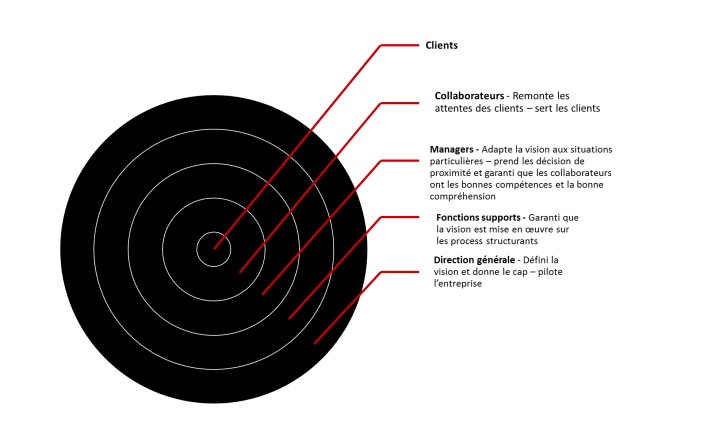
\includegraphics[scale=0.6]{Organisation-circulaire-goji}
\caption{Organisation circulaire Goji, Cadreo}
\label{fig:Goji}
\end{figure}

Pour pouvoir mettre en place ces douze principes. Il est conseillé de passer d'un fonctionnement vertical par un fonctionnement plus neuronal ou circulaire. Ce qui permettra d'avoir le client comme centre d'intérêt principal.  Il est possible de façonner cette organisation type en fonction de la taille et de la structure pour être au plus proche de l'agilité.

\subsection{Les trois vecteurs d'une entreprise agile}

L’agilité se matérialise par une orientation « services » et s’organise par la conjonction de trois vecteurs :\\
\begin{itemize}
\item La motivation rationnelle des ressources humaines : À toutes les étapes de la mise en œuvre de cette notion de « service », l’agilité introduit un mode de travail collaboratif et le partage des responsabilités. Pour être plus flexible, efficace, rapide et pour avoir toujours de l’avance sur ses concurrents, le développement d'une organisation apprenante. Il s'agit de mettre le salarié au centre de la réflexion, de le considérer comme un partenaire privilégié dans l'acquisition d'un avantage concurrentiel. Ensemble, ils apprennent de leurs erreurs.\\
\item L’usage intensif des nouvelles technologies : L’informatisation du SI à permis des gains important en agilité, mais à induit une préoccupation de plus pour les entreprises : la veille technologique. L’informatique fait partie du domaine des technologies et à ce titre évolue rapidement. Tout nouveau logiciel n’apporte pas un gain flagrant par rapport aux anciens. Mais il ne faut malgré tout pas se laisser distancer sous peine de voir ses performances ou ses possibilités être très inférieurs à ce dont sont capables les concurrents. L’approche agile se révèle particulièrement adaptée aux projets actuels impliquant la mise en œuvre de nouvelles technologies. En remettant en question le cycle de vie des projets afin qu’il s’adapte à la durée de vie des applications.\\
\item Des processus reconfigurés en continu : La recherche d’agilité des entreprises les oblige à réagir aussi bien aux événements externes imposés par l’environnement, qu’internes. Au lieu de continuer à poursuivre les objectifs traditionnels de l’ingénierie des systèmes c’est-à-dire la reproductibilité (réutilisabilité) et la prévisibilité, avec l’agilité l'accent est mis sur l’adaptabilité, la qualité et la création de valeur.\\
\end{itemize}

\begin{figure}[h!]
\centering
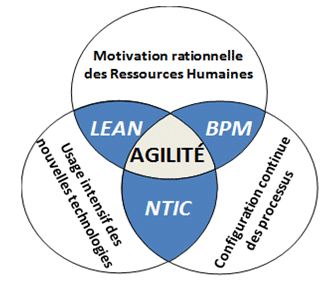
\includegraphics[scale=0.95]{ComposantesAgilite}
\caption{Les 3 vecteurs de l'entreprise agile}
\label{fig:vecteur}
\end{figure}

\subsection{L'agilité et ses différents niveaux}

Ces 12 principes mettent en évidence 3 niveaux d’agilité 
\begin{itemize}

\item[$\bullet$] Agilité technique : Les services deviennent de plus en plus complexe et volumineux. Les services traitent un nombre plus important d’informations. Cet accroissement de taille a fait apparaître le besoin de modifier ou changer rapidement d’une architecture. Les concepts tels que la programmation Objet et l’urbanisation du SI permettent d’accroître l’agilité d’un SI.\\

\item[$\bullet$] Agilité organisationnelle : C’est la capacité à regrouper et encadrer les acteurs métiers et techniques nécessaires à la réalisation du projet. Et cela en dépit des contraintes hiérarchiques. Pour cela plusieurs formes d’organisations possibles :\\

\begin{itemize}

\item Organisation matricielle :\\
Les directions métiers et le directeur de projet sont co-responsables de la performance du projet.
Chaque équipe est composée d’une personne métier relative à sa direction.

\begin{figure}[h!]
\centering
\includegraphics[scale=1]{"orga matricielle"}
\caption{Organisation matricielle}
\label{fig:matrice}
\end{figure}

\item Organisation commando : \\
Il s’agit de regrouper de manière occasionnelle des personnes ayant des compétences ou des connaissances permettant l’aboutissement du projet.
Les intervenants ne dépendent plus de leur hiérarchie métier mais directement du chef de projet.

\begin{figure}[h!]
\centering
\includegraphics[scale=1]{"orga_matricielle2"}
\caption{Organisation Commando}
\label{fig:commando}
\end{figure}

\item Organisation adhocratique :\\
Dans ce type d’organisation il n’existe pas de structure métier. Des spécialistes sont réunis dans des groupes projets. Le directeur de projet est totalement autonome.

\begin{figure}[h!]
\centering
\includegraphics[scale=0.9]{"orga_matricielle3"}
\caption{Organisation Adhocratique}
\label{fig:adho}
\end{figure}

\end{itemize}


\item Agilité fonctionnelle : 
L’enjeu de cette forme d’agilité est de répondre au mieux aux besoins clients et d’intégrer les valeurs d’équipe, de communication et d’acceptation du changement. Il faut regrouper les acteurs appartenant au périmètre projet ou de mettre en place des moyens de communication adaptés pour les acteurs distants géographiquement.\\


\end{itemize}


L'agilité apportent donc des avantages en termes de management d’un groupe projet et en satisfaction client. Ces effets bénéfiques ont poussé les grandes entreprises à les mettre en place. Nous allons voir maintenant quelques exemples d’application de ces méthodes.
\newpage
\subsection{Exemples d’application} 
(Source : Article les echos, 2014)

\begin{figure}[h!]
\centering
\includegraphics[scale=0.2]{"amazon-com-logo"}
\caption{Logo Amazon}
\label{fig:amazon}
\end{figure}

« Amazon représente un exemple d'agilité. Loin de chercher à se reposer sur ses lauriers, l'entreprise pure player remet sans cesse en cause son modèle de fonctionnement pour proposer de nouveaux services ou améliorer les existants, toujours en réponse aux besoins exprimés par ses clients.
Cela s'est traduit par une diversification de l'offre : aux livres, qui constituaient son produit d'appel, Amazon a peu à peu ajouté au sein de son offre d'autres produits facilement livrables par la poste comme des objets high-tech ou du petit électroménager. Résultat : début 2014 l'entreprise de Jeff Bezos pouvait se vanter de réaliser plus de 130 000 dollars de chiffre d'affaires… par minute ! »
\\

Tandis que nous avons des entreprises qui ne se sont pas mis à jour comme a pu le constater la société de téléphonie Nokia. En voici un contre exemple.\\


\begin{figure}[h!]
\centering
\includegraphics[scale=0.4]{"nokia-logo1"}
\caption{Logo Nokia}
\label{fig:nokia}
\end{figure}

« Prenons Nokia, le fabricant Finlandais de mobiles. En 1998 Nokia devient le premier constructeur de téléphones mobiles au monde, et entame les années 2000 avec le vent en poupe. Mais les choses vont se gâter par la suite : faute d'avoir su jauger son marché cible et ses clients, Nokia passe à côté du virage du smartphone, et laisse à Apple le monopole du smartphone dès le lancement de l'I Phone en 2007 : la stratégie de Nokia repose alors encore sur le portable low-cost. En 2011, pour avoir su aller chercher Apple sur son terrain, Samsung lui ravit le titre de premier constructeur de mobile au monde. »\\

L'agilité d'un service amène une certaine facilité d'organisation dans une entreprise et c'est ce qui peut rendre l'entreprise agile. Lors d'une transformation, l'agilité d'une entreprise va rendre cette réorganisation facile. Voyons maintenant ou se place l'agilité vis à vis de la transformation.

\newpage

\part{Interaction entre Agilité et transformation}

Depuis toujours l’entreprise cherche à répondre rapidement, à la meilleure qualité possible et à moindres coûts à la demande du client. C'est-à-dire satisfaire son client. L’entreprise cherche également à avoir des nouveaux clients, en passant par de la différentiation ou de l’innovation. Une entreprise est agile lorsqu’elle est capable d’anticiper les changements, de les compenser dynamiquement, puis de les intégrer.
\setcounter{section}{0}
\section{Processus étudiés, transformation et agilité}

\subsection{L'impact d'une transformation sur l'agilité pendant le temps de la transformation et après}

En général, une certaine inertie est présente pendant la transformation ce qui permet de garder l'agilité du service. Cela seulement lorsque le service est agile. Par contre s'il n'est pas agile, le service ne gagnera pas plus en agilité. Chez Philips dans le data management qui est un service agile, ils essaient de cadrer un peu plus car il y a un problème de charge de travail et pour palier à cela ils tentent de mettre en place un système de « Demand management ». C'est a dire, lorsque le projet arrive, il sera mis dans une liste en mettant des priorités et les ressources dont ils ont besoins. Ce qui entraîne une petite perte en agilité, en contre partie il gagne en standardisation ou en harmonisation sur la façon de traiter la demande.
Or, la transformation entraîne du changement ce qui implique pour ceux qui le subissent de s'y adapter en acceptant et en évoluant vers cette nouvelle situation.\\

Cette courbe du changement passe par plusieurs étapes. On peut voir qu'il y a deux grandes phases : 

\begin{itemize}
\item Pour commencer, une phase descendante qui s'accompagne d'une attitude négative et contre-productive, tournée vers le passé et le refus

\item Par la suite on aura la phase ascendante où ici l'attitude sera productive et tournée vers le futur et le positif.
\end{itemize}

\begin{figure}[h!]
\centering
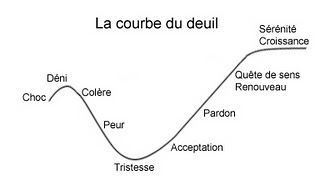
\includegraphics[scale=0.8]{courbe_deuil}
\caption{Courbe du changement}
\label{fig:courbe_chang}
\end{figure} 
\newpage
Le changement apparaît tous les jours, toute la vie, tout change tout le temps. L'homme change tout le temps, donc le changement c'est quelque chose que l'être humain connaît très bien et avec lequel il est très à l'aise, personne n'est angoissé de grandir lorsqu'on est enfant. L'humain peut être angoissé par la mort mais pas par le fait d'évoluer. Et la où est l'erreur humaine c'est d'avoir peur de perdre quelque chose. Lors d'une réorganisation ou d'une transformation la peur est de perdre son voisin avec qui on s'entend bien, de perdre son titre, la reconnaissance de ses collègues, ne plus utiliser l'outil habituel, de changer de scope\footnote{Périmètre} qui est lié à la reconnaissance de compétence, de ne plus être compètent du jour au lendemain, tout comme perdre son portefeuille de clients, etc. Donc le risque de repartir depuis le début. Or lorsqu'on est dans le « continuous improvement », on est mieux équipé pour gérer le changement. L'objectif d'une transformation est d'avoir une meilleure courbe de changement.\\
C'est la performance de l'entreprise et la motivation des employés qui va être impacté par la transformation plus que par l'agilité. Une entreprise ou un service qui n'est pas du tout agile va avoir quelques difficultés lors de la transformation. Car il serait probable qu'ils ne sachent pas gérer cette situation.\\

\newpage

Lors d'une transformation il faut prendre en considération les différents périmètres pour mener à bien une réorganisation. C'est en associant ces trois périmètres de façon correct que la restructuration sera réussie.\\

\begin{figure}[h!]
\centering
\includegraphics[scale=0.45]{"Diapositive2"}
\caption{Schéma périmètre}
\label{fig:scope}
\end{figure}


Voici les 3 périmètres : \\ 

\begin{itemize}

\item Le premier périmètre est le périmètre principal le « Système formel », cela va être une étape que font les personnes systématiquement lors d'une réorganisation. On peut prendre en exemple Philips ici le service du data management, qui eux explique tout d'abord la stratégie, ensuite la raison du changement, par la suite la nouvelle organisation, la répartition des tâches des employé et enfin à quel endroit seront-ils postés. Tout ceci est très rationnel, cela s'appelle « l'organisation design ». Ce système fait partie du cadre de l'organisation « L'organization framework » .\\
\end{itemize}
Tandis que les deux autres système font parties de l'« Individual Mindset Contributing To New Collective Models » qui va permettre de savoir comment chaque personne, avec un bon état d'esprit, va contribuer à créer de nouveau modèle pour tout le monde \footnote{Un modèle collectif}. Et la condition pour avoir cette partie, c'est qu'il faut être agile.\\

\begin{itemize}
\item Le second est le « Système culturel ». Qui lui va permettre de se forger une identité. Ici nous allons reprendre l'exemple de Philips lighting à propos de l'équipe du data management qui est devenu EIM\footnote{Enterprise Information Management}. Or avant l'équipe data management et l'équipe IM\footnote{Information Management} ne travaillaient jamais en collaboration, donc l'objectif était de donner une identité commune à toutes les deux en les fusionnant. Et pour cela il faut prendre en considération l'histoire de ces deux équipes. Il faut construire la culture EIM qui n'existait pas avant. Ce n'est pas qu'il a fallu la construire de zéro mais comme la majorité des personnes venaient de IM, il a fallu s'assurer que les gens de IM deviennent EIM plus que data management devienne EIM car la majorité venaient d'Information Management. Que IM comprenne qu'il fallait pas qu'il continue a faire ce qu'il faisait avant en tant qu'IM parce qu'il n'était plus entre eux. Et qu'il fallait prendre en compte le travail que faisait l'équipe du data management. \\

\item Et enfin le « Système Social » qui lui va permettre de savoir comment on va travailler. Une fois de plus nous allons prendre le cas Philips ainsi que son service du data management. Il y a des « Domaine lead », dans des operations région, avant tout le monde était dans la même équipe maintenant se sont des équipes différentes, et des chef diffèrent. Maintenant il essaie de mettre en place des règles de collaboration et des tableaux. Comme par exemple le RACI qui est l'acronyme de « Responsible, Accountable, Consulted and Informed », dans le management, elle représente une matrice des responsabilités qui fait quoi, qui est responsable de quoi, comme vous pouvez le voir dans la figure \ref{fig:raci}.\\

La confrontation c'est l'action de confronter des personnes, de les mettre face à face. Chez philips lighting un chef d'équipe va être impliquer dans un projet, en temps normal c'est le domaine expert qui doit être impliqué dans ce type de projet, or le responsable du service ne voulant pas lui octroyer trop de responsabilité, voulait lui donner le projet sans pour autant lui rajouter le rôle de domaine expert. Si le projet ce déroule bien personne ne sera sollicité. Or s'il y a un moindre soucis et qu'il faut « escalader », et bien s'il le fait en tant que « Team lead » il remontra vers le responsable du service, alors que s'il le fait en tant que domaine expert. Il passera par le responsable du domaine. Donc le résultat n'est pas le même. On peut dire que les designs sont établis pour les problèmes donc il est très important de formaliser tous ça, en confrontant les différents acteurs.\\
Enfin, il faut prendre en considération les contraintes des différentes règles qui ont été mise en place pour travailler sur la transformation. \\
\end{itemize}


\begin{figure}[h!]
\centering
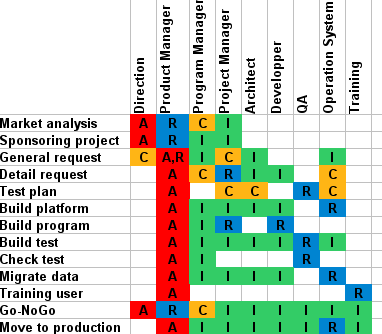
\includegraphics[scale=0.7]{raci}
\caption{Tableau RACI}
\label{fig:raci}
\end{figure}

L'agilité d'une entreprise va permettre de faire toutes ces actions de façon rapide, tandis qu'une entreprise qui n'est pas agile va seulement faire le côté formel parce qu'elle n'est pas équipée, ce qui risque d'engendrer des conflits. On passe d'une étapes où l'on travaille d'une manière à une étape ou l'on doit apprendre a travailler d'une autre façon. Et cela prends du temps. Grâce a ceci les employés apprennent a travailler autrement. La décision ne sera pas prise d'en haut, elle le sera faite par les employés. Qui plus est si l'entreprise est agile, les personnes qui l'occupe ont les compétences et le bon état d'esprit pour ce poser les bonnes questions et faire des formalisations. L'agilité va permettre d'en sortir plus vite.\\ 
 
Beaucoup d'entreprise font une réorganisation sans prendre en compte le coté culturel et social. Or en ignorant ces périmètres, ils continueront à faire la même chose. Donc ils auront changé la stratégie, la structure et le management pour au final avoir un même rendu. Les gens parle de réorganisation mais en faites s'il ne prennent pas la transformation globale en compte, et bien ils vont à l'échec.\\

\subsection{La possible régression de l'agilité par la transformation}

La transformation va apporter des modifications dans un service, que ce soit organisationnelle ou au niveau des outils utilisés au sein du service, ce qui amènera à mettre en place de nouveaux processus et aussi de réattribuer certain poste. En faisant ceci, les tâches seront conservées ou redistribuées aux personnes concernées. 

Durant cette transformation chez Philips, il y a eu différents domaines qui ont été créés, les interactions entre les équipes ont rencontré quelques complications suite à ces différents changement. L'une des raisons est dû aux ressources. Un employé risque de se retrouver à cumuler la tâche qu'il effectuait auparavant ainsi que la nouvelle, car il a fallu laisser le temps que la nouvelle personne nommée pour cette tache soit opérationnelle. L'autre raison qui découle de la première, est la perte de communication, des échanges inter-équipes qui ne sont pas encore reformalisé comme il se doit. De plus l'autre cause que j'ai pu constater que Philips standardise l’exécution de ses processus via son ERP\footnote{ERP (Enterprise Resource Planning) est un système d’information qui permet de gérer et suivre au quotidien, l’ensemble des informations et des services opérationnels d’une entreprise.} en imposant ses outils informatiques. Ici l'ERP utilisé est SAP. Ceux-ci obligent les utilisateurs à s’adapter et à adapter les processus.\\

Toutes les entités de Philips utilisent SAP, dans toutes les divisions et cela dans le monde entier. L’organisation entière de Philips est orientée sur SAP. Et il n’y a pas d’exception. Lors de l’acquisition d’une nouvelle entreprise après avoir rattaché les nouveaux employés à l’organigramme et réorganisé le management, commence le projet d’intégration de la nouvelle entité dans SAP. Même si cela implique une régression technologique pour les nouveaux arrivants.\\ 

On a comme exemple récent l’acquisition d'une nouvelle fonctionnalité dans l'ERP SAP. Ce nouvel outil est SAP HANA\footnote{SAP HANA est un SGBD relationnel In-Memory en colonnes.}. Il a vu son intégration dans SAP débuter il y a de cela 3 mois et il est toujours en cours. Il permettra d'éviter de lier des données SAP avec d'autre logiciel ainsi qu'une éventuelle possibilité d'optimiser les traitements de données.\\
En utilisant cette nouvelle fonctionnalité tout sera centralisé dans L'ERP SAP. Mais en contre partie le service du data management a dû adapter ses processus aux possibilités offertes par SAP. Ce qui a entrainé à la fois une régression technologique pour le service ainsi qu’une perte d’agilité vis-à-vis de leurs clients. Ils sont passés d’un système SQL server dont ils avaient entièrement le contrôle à un système qui est centralisé.\\
Donc nous pouvons dire que le fait de standardiser, d'harmoniser ou d'uniformiser fait perdre l'agilité et pour cela il faut trouver un juste milieux.

\subsection{Ressources et compétences d'un service agile qui peuvent permettre une transformation réussie}

\subsubsection{L'accompagnement}

Lorsque la transformation est bien accompagnée, nous irons au delà du progrès et nous allons rentrer dans une organisation qui sera une entreprise agile car les gens auront appris a prendre du recule et ceci est dû au faite qu'ils savent se transformer pour tous les jours parce qu'ils font du « continuous improvement », ils vont très vite remonter d'après la courbe du changement. Il est utopique d'avoir une courbe qui ne fait que croître.\\
\newpage
\begin{figure}[h!]
\centering
\includegraphics[scale=0.55]{"Diapositive1"}
\caption{Courbe d'amélioration}
\label{fig:courbe}
\end{figure}

\begin{itemize}
\item Concernant la courbe du milieux. Si une équipe de consultant vient s'occuper de la transformation celle ci sera réalisé mais ne pourra être durable car les gens ne seront pas pilote du changement. Ils ne seront pas responsabilisés. Ce qui les amènera à réapprendre suite à cette transformation.\\
\item Tandis que le coach, ici la courbe la plus haute, va être là pour accompagner le manager. Il sera à ses cotés pour l'assister en tant que binôme. Cette méthode va permettre de les faire grandir plus rapidement.\\
\item Enfin, pour la dernière courbe. S'il n'y a pas du tout d'accompagnement du changement, la « Bouillie de chenille » durera beaucoup plus longtemps. Le risque est qu'il y ai une incertitude du résultat. Il pourrait même être possible qu'on n'atteigne pas le niveau initial. Ici on ne parlera même pas de progrès mais de régression.\\
\end{itemize}

Le changement doit s'accompagner s'il ne l'ai pas nous ne savons pas où nous allons. Si l'entreprise est agile la courbe du changement se fera plus rapidement car les gens auront les bon réflexe car ils sont formés au changement, le changement fera partie intégrante de leur vie. Ils auront une culture du changement. Or si l'agilité est bien mature, celle-ci sera une ressource pour la transformation, elle aidera la transformation. Mais une entreprise qui est déjà agile est assez mature pour savoir gérer une transformation. Il y aura un moment ou l'agilité sera impacté car on sera dans la phase de « bouillie de chenille » mais celle-ci remontera. 

\subsubsection{La culture}

L'agilité va apporter un changement fondamentale dans la façon de penser. Or beaucoup d'entreprise considère que l'agilité est un produit à acheter ou à vendre. Les entreprise qui ont un « Time to Market »\footnote{Délai de mise sur le marché} trop lent veulent une solution rapide. Pour que ces entreprises réussissent sur le long terme, ils doivent penser à l'agilité comme une culture et non comme une marchandise. En conséquence, la culture de l'entreprise ainsi que celle de l'employé joue un rôle déterminant sur l'agilité.\\
La société Philips pour faire émerger sa culture a mis en place le « Lean management » car ils sont dans un contexte où la charge de travail augmente, aussi qu'il est difficile d’avoir des ressources supplémentaires, que la concurrence est importante et qu'il y a une guerre des prix, de plus que les coûts de production sont élevés, enfin qu'il y a une volonté d’améliorer la rentabilité de l’entreprise. Cela nécessite de mettre en place une démarche d’amélioration continue des performances. Par conséquent, la société a mis en place au sein de ses services une démarche de type Lean Management.\\
Ce « Processus qui recherche la performance de l’entreprise par la suppression des gaspillages, dans le but de respecter les exigences du client en termes de qualité, coûts, délais et réactivité ».  Le lean est plus qu’une amélioration continue d’un processus mais un état d’esprit, tout comme l'agilité. Elle se déploie dans tous les secteurs d’activité. Le data management l'a adopté depuis plus de 3ans. Elle utilise entre autre la méthode du 5S qui va lui permettre d'éviter le gaspillage et d'éliminer les causes de plusieurs petits problèmes, voir la figure \ref{fig:5s}. \\
Les lettres correspondent au premiére lettre de ces cinq termes japonais :
\begin{enumerate}
\item seiri : sort (trier)
\item seiton : set in order (ranger)
\item seiso : shine (nettoyer)
\item seiketsu : standardise (standardiser)
\item shitsuke : sustain (respecter)
\end{enumerate}
Elle a adapté cette méthode en ajoutant un sixième «S». Il correspond au «S» de Safety. C'est l'une des premières méthodes à mettre en œuvre dans une démarche de lean management. Elle va aider aussi à changer la mentalité des employés. Par conséquent, les salariés auront acquis une culture d'entreprise. Cette démarche a fait ses preuves dans l’amélioration de la performance.\\
Pour émerger cette culture au sein de l'entreprise. La société Philips a mis en place ce processus, et afin d'accélérer la formation de tous ses employés, la compagnie a mis, durant la première année une prime qui était comprise dans la prime d'intéressement. Elle sera calculée en fonction du nombres de personne ayant fait la formation. Ceci permettait de motiver et d'inciter les employés à se former au Lean management. De ce fait, cela permettrait d'avoir une agilité renforcé lors d'une transformation.

\begin{figure}[h!]
\centering
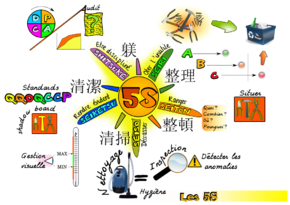
\includegraphics[scale=1]{Carte_5S}
\caption{La méthode 5S}
\label{fig:5s}
\end{figure}


\newpage
\part{Conclusion}

L'agilité d'une entreprise ne s’oppose pas à la transformation de la société, au contraire elle en est même une composante essentielle à une restructuration rapide. Elle permet d’avoir une vue globale des processus et de réutiliser ceux-ci. Mise en place avec un management, poussant les employés à la proposition d’amélioration et de la communication, elles permettent d’avoir une amélioration continue des processus essentielle à l’agilité de l’entreprise.\\

Pour avoir une bonne réorganisation, il faut prendre en considération tous les périmètre d'une transformation. En prenant en considération le périmètre culturel ainsi que le périmètre social.\\

Par contre, lorsque le service standardise ou normalise à l'excès en reconfigurant en continu, que ce soit à l’échelle globale ou locale, cela entraîne un emprisonnement de l’employé à la définition du processus. Il doit le respecter et l’appliquer sans avoir la possibilité de le modifier, de l’améliorer. \\

Chez Philips les causes d’une agilité incomplète sont à rechercher dans la stratégie d’alignement de l’entreprise. Soit celle-ci n’a pas conscience  de la perte d’agilité engendrée par la standardisation et sur les insuffisances du management Lean mis en place, soit elle l’accepte pensant que le coût permettant d’améliorer son agilité n’en vaut pas le prix\\

Malgré tout même si la stratégie globale de l’entreprise ne prend pas en compte la localisation nécessaire à l’agilité, les organisations locales ont les moyens d’ajouter une couche d’agilité à la transformation établis par l’organisation globale.


\newpage
\pagenumbering{Roman}
\setcounter{page}{1}
\part{Annexe}
\listoffigures
\newpage
\setcounter{section}{0}

\appendix
\section{Webographie}

\vspace{0.5cm}
\vspace{0.3cm}

\begin{figure}[h!]
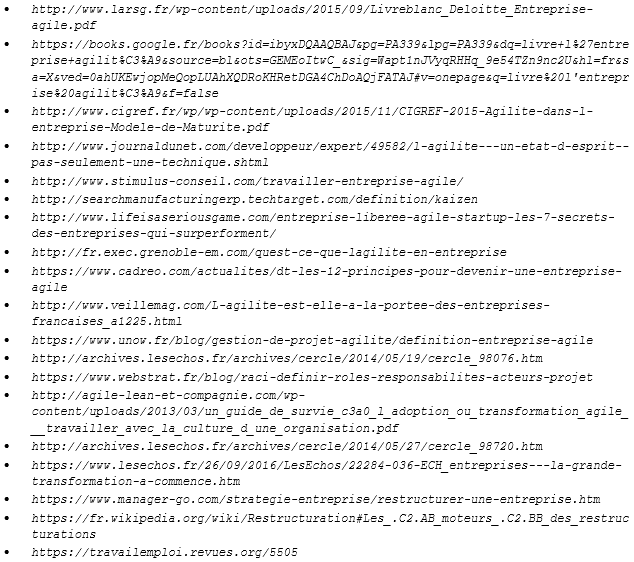
\includegraphics[scale=1.2]{biblio}
\end{figure}

%http://www.zdnet.fr/actualites/outre-l-agilite-le-devops-impacte-la-culture-de-l-entreprise-et-son-organisation-39837950.htm  (solution prez)
%http://archives.lesechos.fr/archives/cercle/2014/05/27/cercle_98720.htm (solution prez)

%http://www.utc.fr/~mastermq/public/publications/qualite_et_management/MQ_M2/2015-2016/MIM_stages/TREHOUR_Nicolas/ST02_2016_Trehour_POSTER_A4.pdf

%http://www.larsg.fr/wp-content/uploads/2015/09/Livreblanc_Deloitte_Entreprise-agile.pdf

%https://books.google.fr/books?id=ibyxDQAAQBAJ&pg=PA339&lpg=PA339&dq=livre+l%27entreprise+agilit%C3%A9&source=bl&ots=GEMEoItwC_&sig=Wapt1nJVyqRHHq_9e54TZn9nc2U&hl=fr&sa=X&ved=0ahUKEwjopMeQopLUAhXQDRoKHRetDGA4ChDoAQjFATAJ#v=onepage&q=livre%20l'entreprise%20agilit%C3%A9&f=false
%http://www.cigref.fr/wp/wp-content/uploads/2015/11/CIGREF-2015-Agilite-dans-l-entreprise-Modele-de-Maturite.pdf

%http://www.journaldunet.com/developpeur/expert/49582/l-agilite---un-etat-d-esprit--pas-seulement-une-technique.shtml

%http://www.stimulus-conseil.com/travailler-entreprise-agile/

%http://searchmanufacturingerp.techtarget.com/definition/kaizen

%http://www.lifeisaseriousgame.com/entreprise-liberee-agile-startup-les-7-secrets-des-entreprises-qui-surperforment/

%http://fr.exec.grenoble-em.com/quest-ce-que-lagilite-en-entreprise

%https://www.cadreo.com/actualites/dt-les-12-principes-pour-devenir-une-entreprise-agile

%http://www.veillemag.com/L-agilite-est-elle-a-la-portee-des-entreprises-francaises_a1225.html

%https://www.unow.fr/blog/gestion-de-projet-agilite/definition-entreprise-agile

%http://archives.lesechos.fr/archives/cercle/2014/05/19/cercle_98076.htm

%https://www.webstrat.fr/blog/raci-definir-roles-responsabilites-acteurs-projet

%http://agile-lean-et-compagnie.com/wp-content/uploads/2013/03/un_guide_de_survie_c3a0_l_adoption_ou_transformation_agile___travailler_avec_la_culture_d_une_organisation.pdf

%http://archives.lesechos.fr/archives/cercle/2014/05/27/cercle_98720.htm

%https://www.lesechos.fr/26/09/2016/LesEchos/22284-036-ECH_entreprises---la-grande-transformation-a-commence.htm

%https://www.manager-go.com/strategie-entreprise/restructurer-une-entreprise.htm

%https://fr.wikipedia.org/wiki/Restructuration#Les_.C2.AB_moteurs_.C2.BB_des_restructurations

%https://travailemploi.revues.org/5505

\end{document}

